\documentclass[conference,flushend]{iaria} % (based on IEEEtran.cls)
% The class iaria.cls loads biblatex/biber with correct IARIA settings
% as well as a set of common packages (times, inputenc[utf8], fontenc[T1],
% graphicx, xcolor, url, orcidlink, hyperref, extdash[shortcuts])

\usepackage{subfigure}

\addbibresource{references.bib}
\title{Minimal Working Example of an IARIA Paper}
\author{
  \IEEEauthorblockN{%
    Jakob Löw\orcidlink{0009-0006-7088-8684}, Kevin Mayer\orcidlink{0000-0002-5597-3913}, Hans-Joachim Hof\orcidlink{0000-0002-6930-9271}}
  \IEEEauthorblockA{%
    CARISSMA Institute of Electric, Connected and Secure Mobility \\
    University of applied sciences Ingolstadt \\
    Ingolstadt, Germany \\
    e-mail: {\tt$\lbrace$jakob.loew\,|\,kevin.mayer\,|\,hof$\rbrace$@thi.de}
} }
\begin{document}
\maketitle
\begin{abstract}
This paper is a minimal working example.
% TODO: copy some parts from expose introduction?
\end{abstract}
\begin{IEEEkeywords}
minimal; MWE; IARIA.
\end{IEEEkeywords}

\section{Introduction}
Many countries are currently transitioning away from combustion engine vehicles towards battery electric ones.
This transition is happening at a rapid rate, because buying an electric vehicle often gets incentivised through tax reductions or straight refunds \cite{stats_electricvehicles}.
With people buying more and more electric vehicles, the demand for charging infrastructure rises.
In Germany not only electric vehicles, but also the buildup of charging infrastructure got heaviliy subsidized by the government.
This high demand and government incentives resulted in a rapid growth in charging station numbers, suppliers and operators \cite{stats_chargepoints}.
Due to the rushed development, the cybersecurity of current charging stations is below average compared to other cyberphysical systems \cite{nasr_power_2022, johnson_review_2022, ahalawat_security_2022}.
Recently cybersecurity researchers investigating charging backend infrastructure have found a range of text book vulernabilities, such as SQL injection, cross site scripting or unauthenticated remote update procedures \cite{nasr_power_2022}.
\\
This paper will focus on fast charging stations. Because of their functionality design, described in a later section, they require a high level direct communication with the vehicle for charging conditions and limits.
While other works such as Tu et al. \cite{tu_extreme_2019} have already covered eletrical and other aspects of fast charging stations, this paper will focus on communication aspects.
The ISO15118 standard was created for communication between charging stations and vehicles, enabling interoperability between stations and vehicles from different manufacturers.
This high level communication protocol provides a larger attack surface compared to other charging techniques, making it more interesting for cybersecurity reserarch.

\section{Charging Station Communication}
Electricity generally comes in two forms: alternating current (AC) and direct current (DC).
While power grids are usually AC, batteries need to be charged using DC.
Therefore the AC needs to be converted to DC either in the car or in the charging station itself.
While cars usually come with an onboard AC to DC converter for charging the onboard battery their power is usually limited between 7 and 22 kW.
In order to achieve higher charging powers, a fast charging station provides a stationary AC to DC converter. Placing it outside of the car removes weight requirements, simplifies cooling and thus allows higher charging currents. \\
In general charging stations can be divided into three categories:
\begin{enumerate}
\item Unmetered AC charging (often used in residential buildings)
\item Commercial AC charging stations
\item DC fast charging stations
\end{enumerate}%
%
The following subsections describe the communication and payment mechanisms of these three kinds of charging stations as well as the included security concepts.

\subsection{Low Level Communication}
AC charging stations usually supply grid power directly, making them just sockets with some very basic communication to the vehicle.
In the early days of electric vehicle adoption mainly these kind of charging stations were built.
Because charging a modern vehicle using an AC charging station can take multiple hours, they usually aren't used for long distance driving.
Because of their low price and low electrical requirements they are however still widely used and newly installed, especially for home and office charging as well as on park and ride parking lots. \\
The by far most common plug for AC charging is the type 2 connector shown in figure \ref{fig:type2}. It is used not only the standard charging plug in Europe, but also in China and other parts of Asia.
Apart from the typical connections of a 3-phase power socket, the connector incorporates two additional pins: charge pilot (CP) and proximity pilot (PP).
These two pins are used for a very simple resistor based signaling scheme defined in IEC 61851 \cite{IEC61851} and explained by \cite{gonium_talk}:
The charging cable includes a resistor between proximity pilot and protective earth (PE), which signals the maximum current for this cable.
The charging station supplies a +12V/-12V pulse width modulation (PWM) signal between CP and PE.
The vehicle contains both a diode and a resistor between CP and PE, such that the charging station can detect the presence of a vehicle based on the negative voltage being dropped by the diode and the positive voltage being reduced by the resistor.
As soon as the vehicle is ready to charge it connects a second resistor between CP and PE further reducing the voltage.
For unmetered AC charging this is sufficient to start a charging session.
For public AC charging infrastructure usually external means of payment, such as mobile app activation or contactless payment have to be used before the charge session is started.
During the charging session the charging station tells the vehicle the maximum allowed current through changing the duty cycle of the +12V/-12V PWM signal between CP and PE.
There exists a special PWM duty cycle of 5\%, which can be used by the charging station to tell the vehicle to use the high level ISO15118 protocol for communication rather than the low level communication described in IEC 61851 \cite{IEC61851}.

\begin{figure}[ht]
    \centering
    \begin{subfigure}
        \centering
        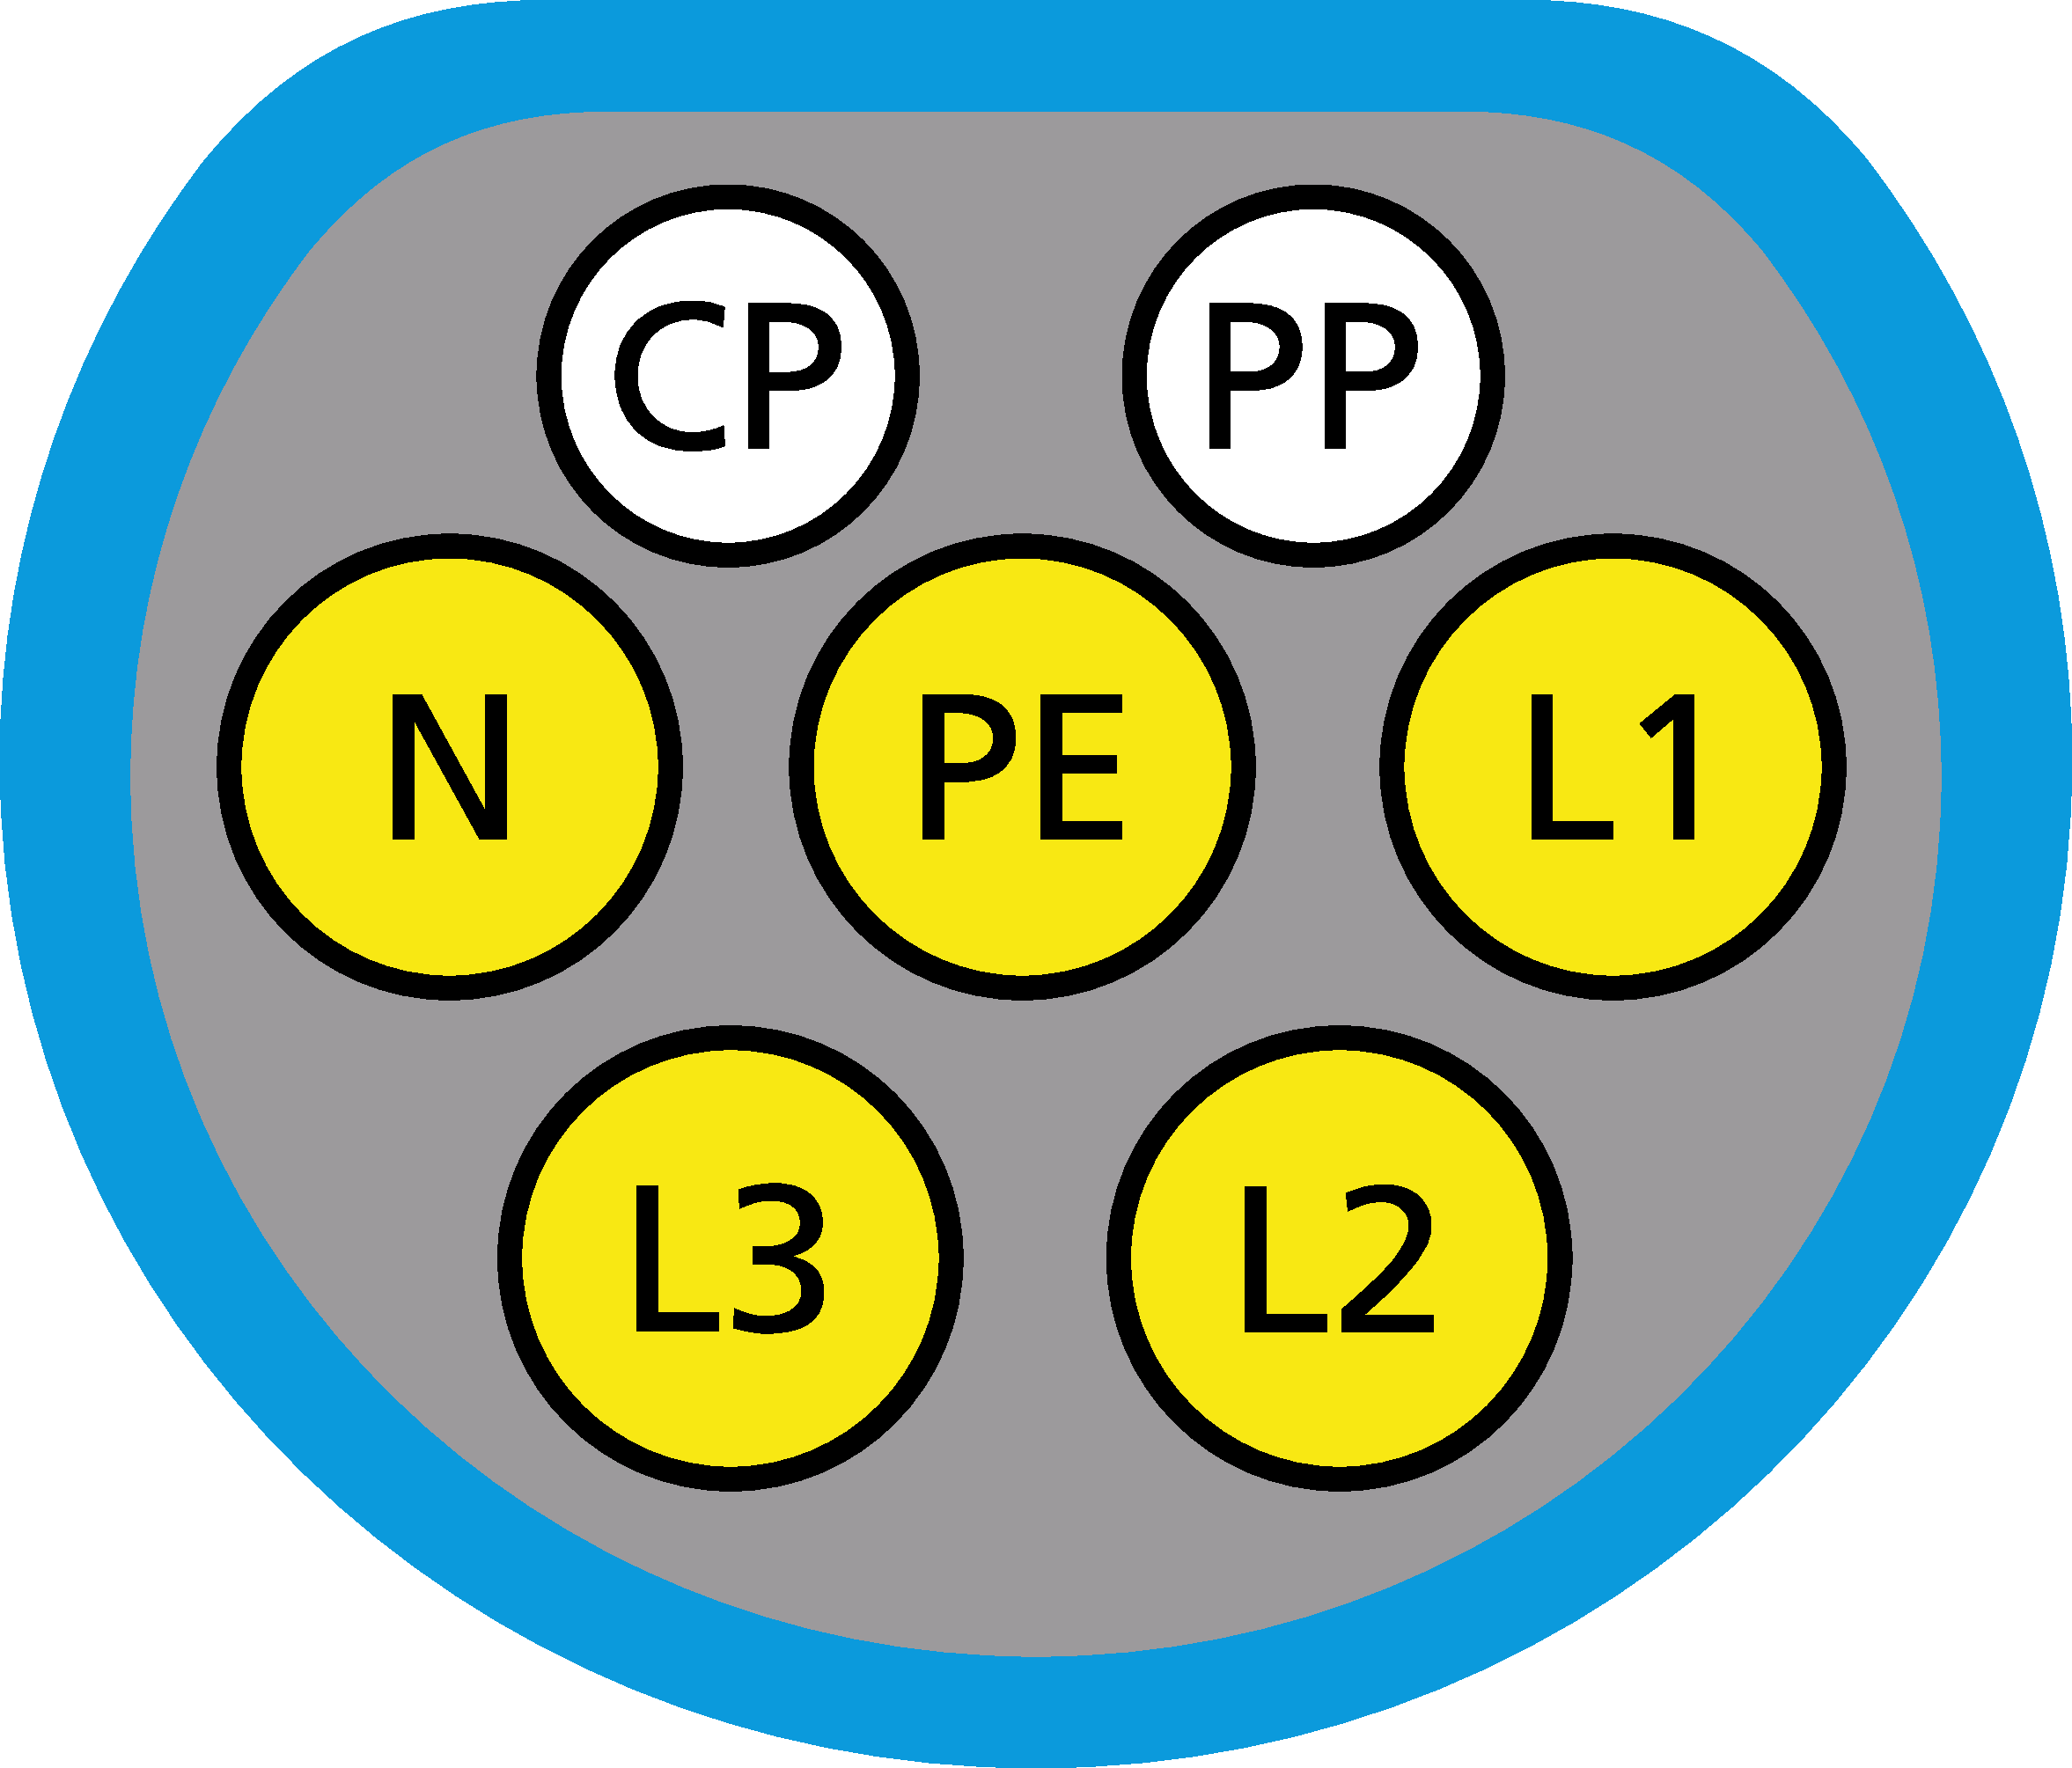
\includegraphics[width=.2\textwidth]{graphs/type2.pdf}
        %\caption{IEC 62196 Type 2 connector schematic}
        \label{fig:type2}
    \end{subfigure}
    \hfill
    \begin{subfigure}
        \centering
        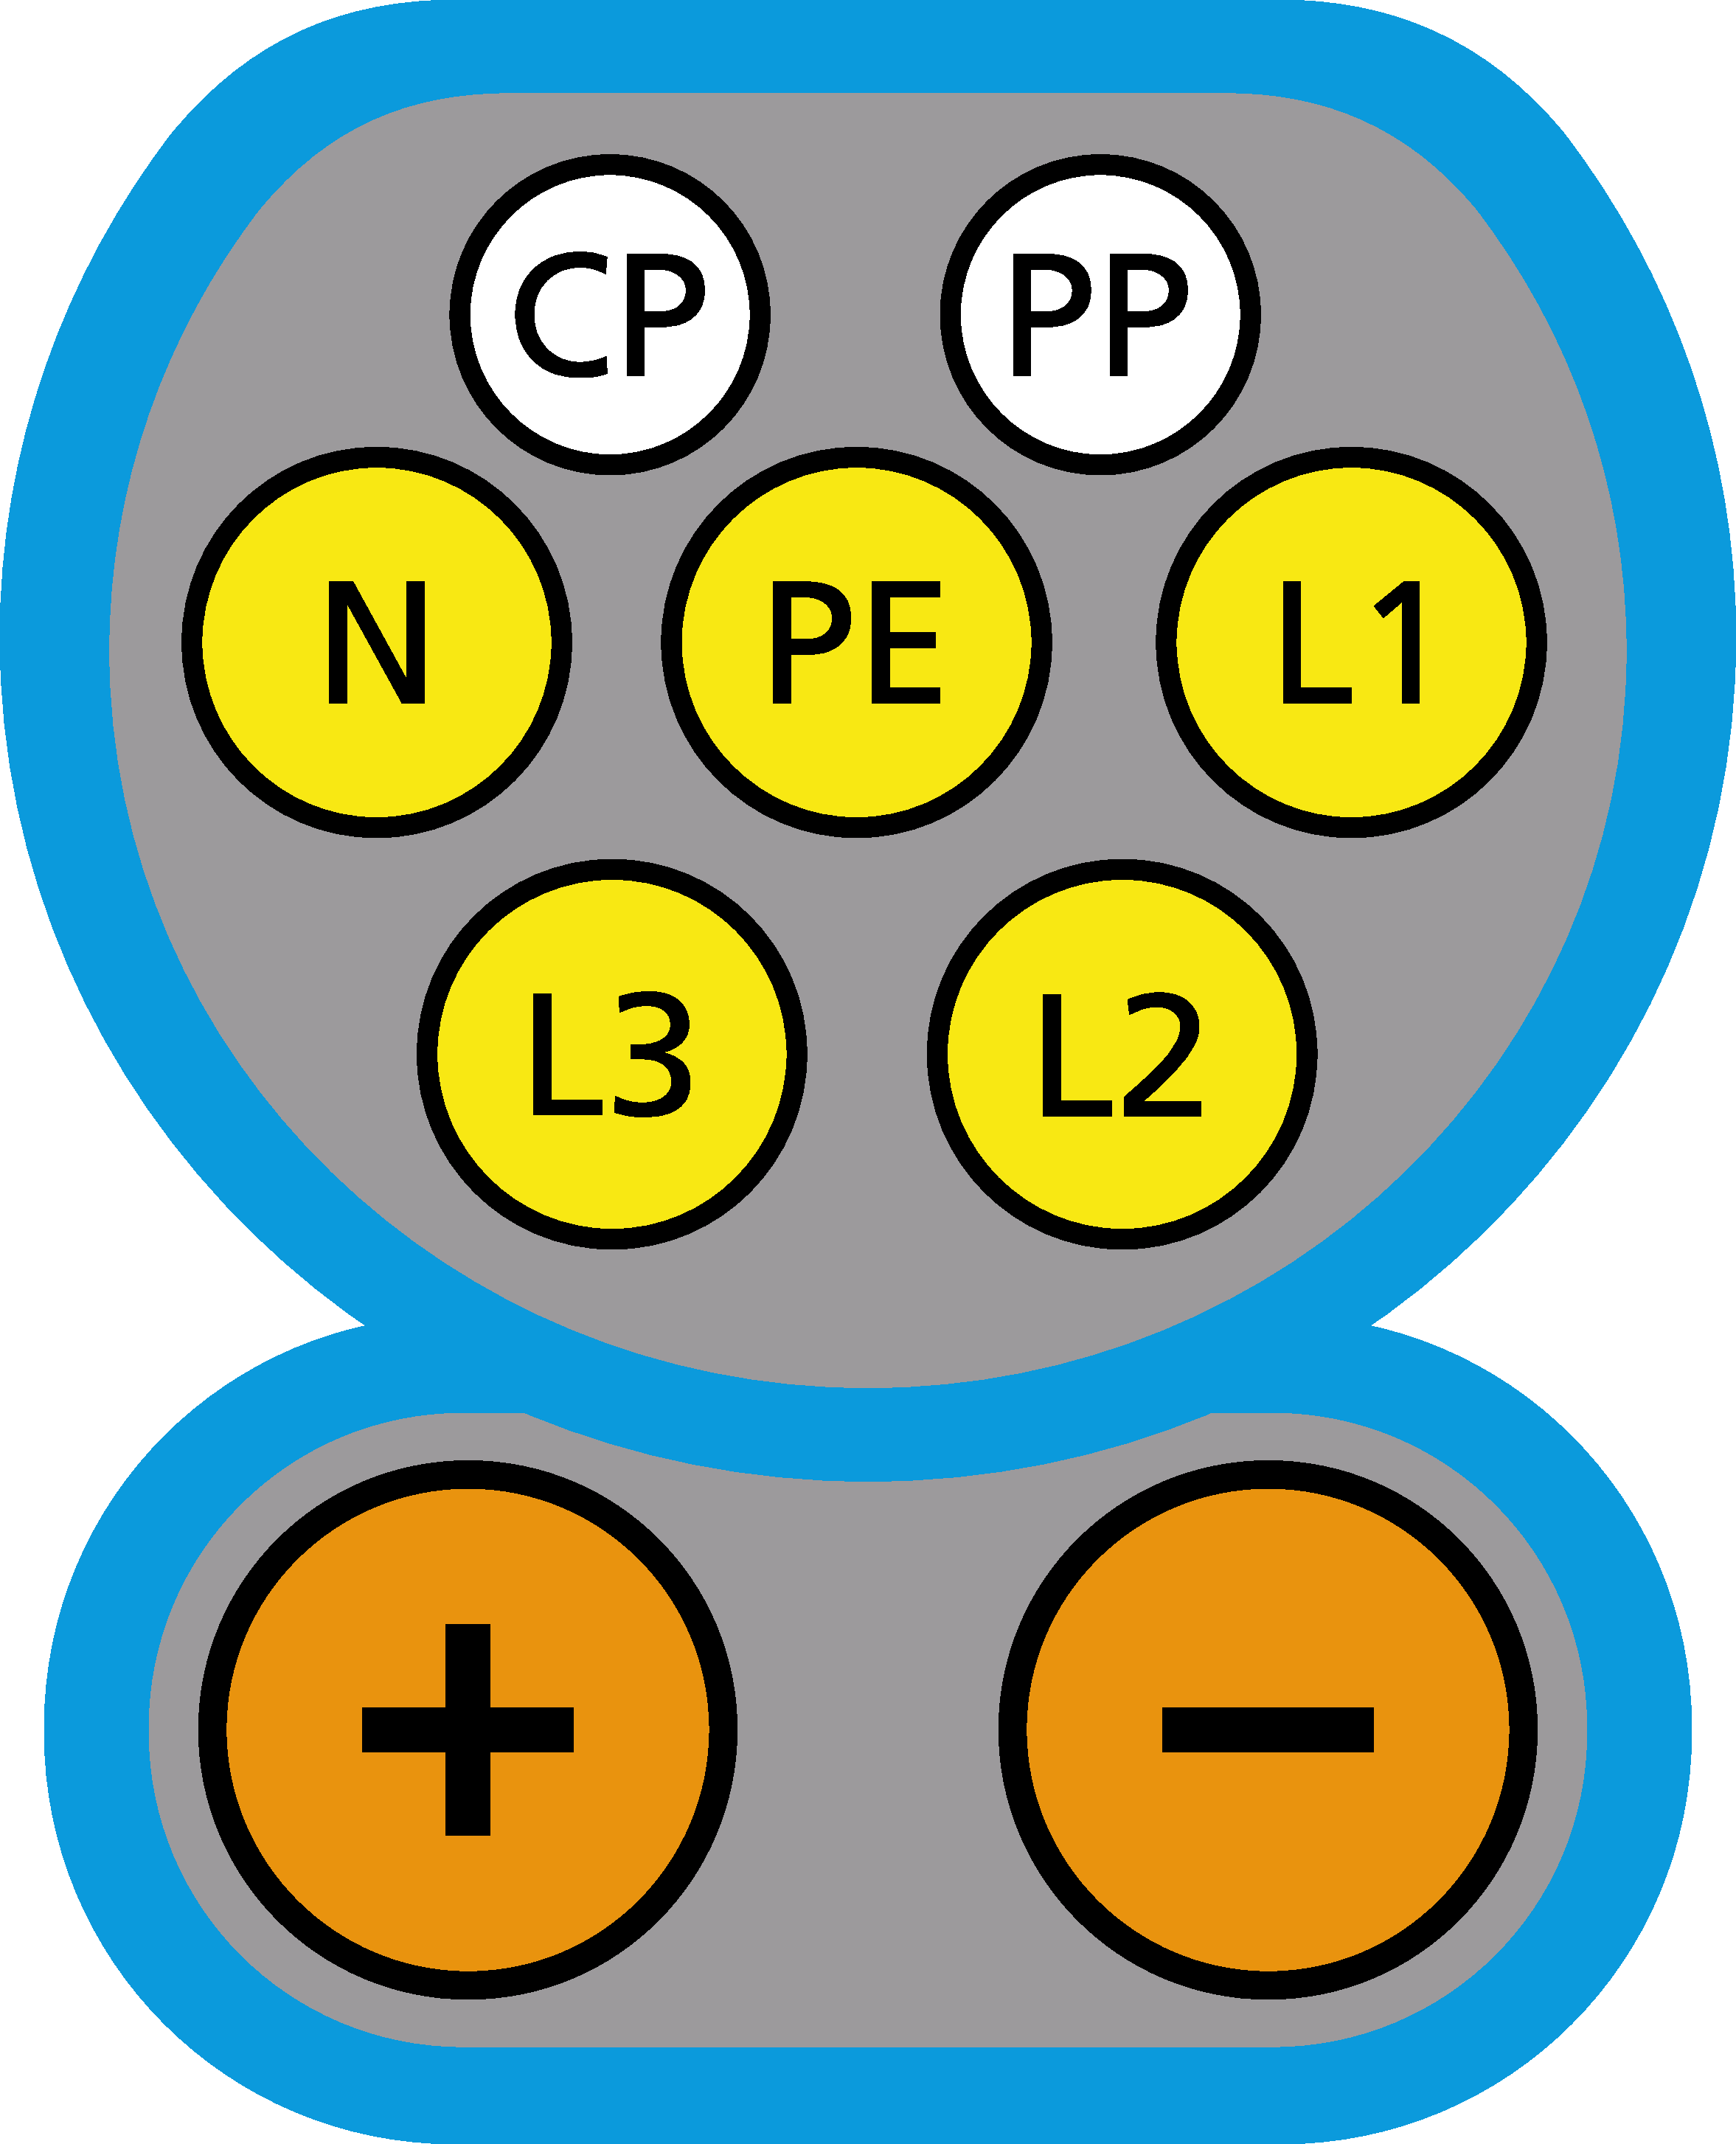
\includegraphics[width=.2\textwidth]{graphs/ccs.pdf}
        %\subcaption{Combined charging system connector schematic}
        \label{fig:ccs}
    \end{subfigure}
    \caption{Schematic diagrams type 2 (left) and combined charging system (right) connectors}
    \label{fig:connectors}
\end{figure}

% refs:
%% \cite{IEC61851} - resistor & PWM communication
%% \cite{gonium_talk} - gonium talk about charging stations: TODO often other vulnerabilities
%% \cite{antoun_detailed_2020} - claims grid communication exists, claims home chargers have high-level communication with vehicles

\subsection{High Level Communication}

\iffalse
DC charging stations on the other hand are required to communicate to the vehicle for properly supplying the correct voltage and power to the battery.
For this high level communication the industry standard ISO15118 was created, enabling interoperability between different vehicle manufacturers and charging station vendors.
While this standard allows possibilities for payment processing and value added services, it also comes with a lot of security implications.
\fi
% TODO extend this

\subsection{ISO15118 Security Concepts}
% TODO: PnC, TLS, TLS-downgrade

\subsection{Other Communication Standards}
% chademo, GB/T, MCS, ...
%% \cite{gonium_talk} - gonium talk about charging stations: TODO often other vulnerabilities
%% \cite{garofalaki_electric_2022} - OCPP security issues and challenges

\section{Charging station technologies and vendors}
%% \cite{das_electric_2020} - EV market share, charging standards list
%% TODO: add vendor market analysis
%% TODO: add charge port analysis
\begin{figure}[ht]
    \centering
    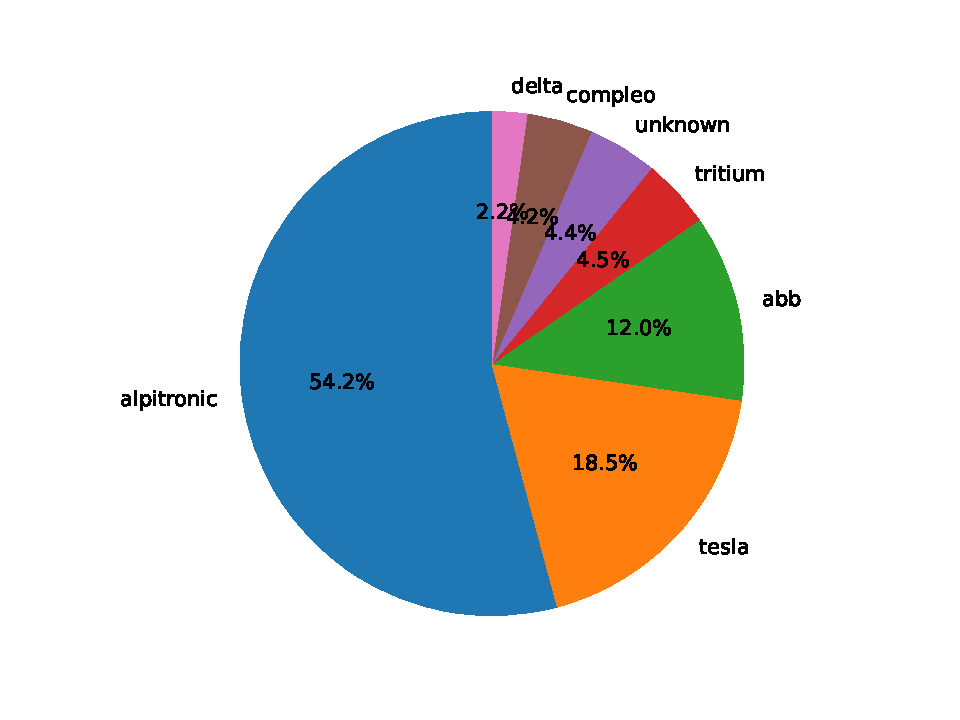
\includegraphics[width=.489\textwidth]{graphs/market_analysis.pdf}
    \caption{CCS charging station vendor market share}
    \label{fig:marketshare}
\end{figure}

\begin{figure}[ht]
    \centering
    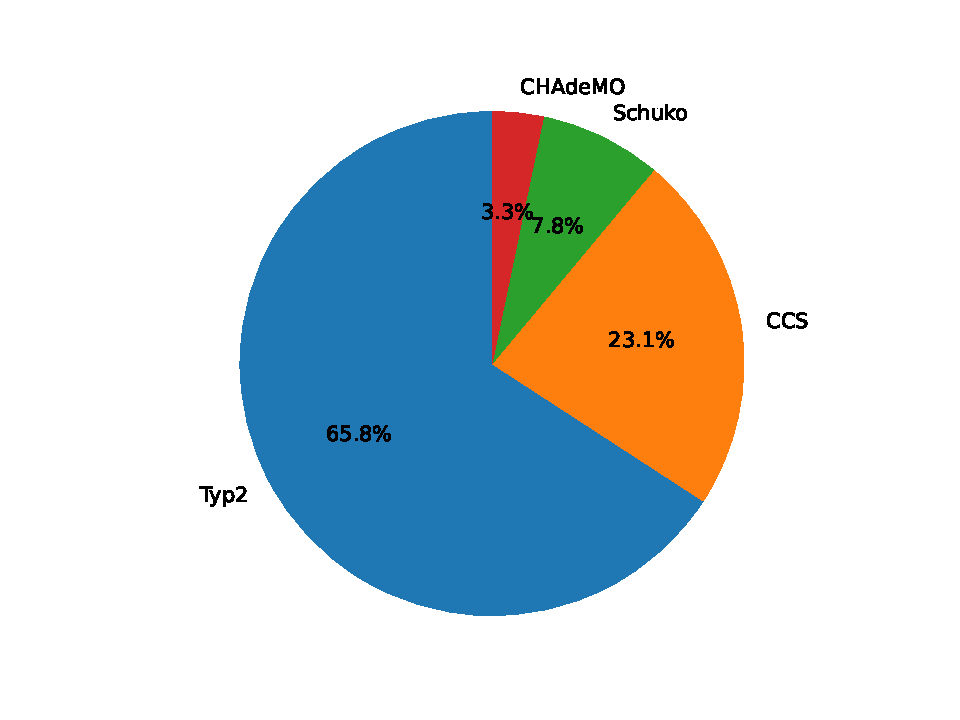
\includegraphics[width=.489\textwidth]{graphs/socket_analysis.pdf}
    \caption{Charging station socket market share}
    \label{fig:sockets}
\end{figure}

\begin{figure}[ht]
    \centering
    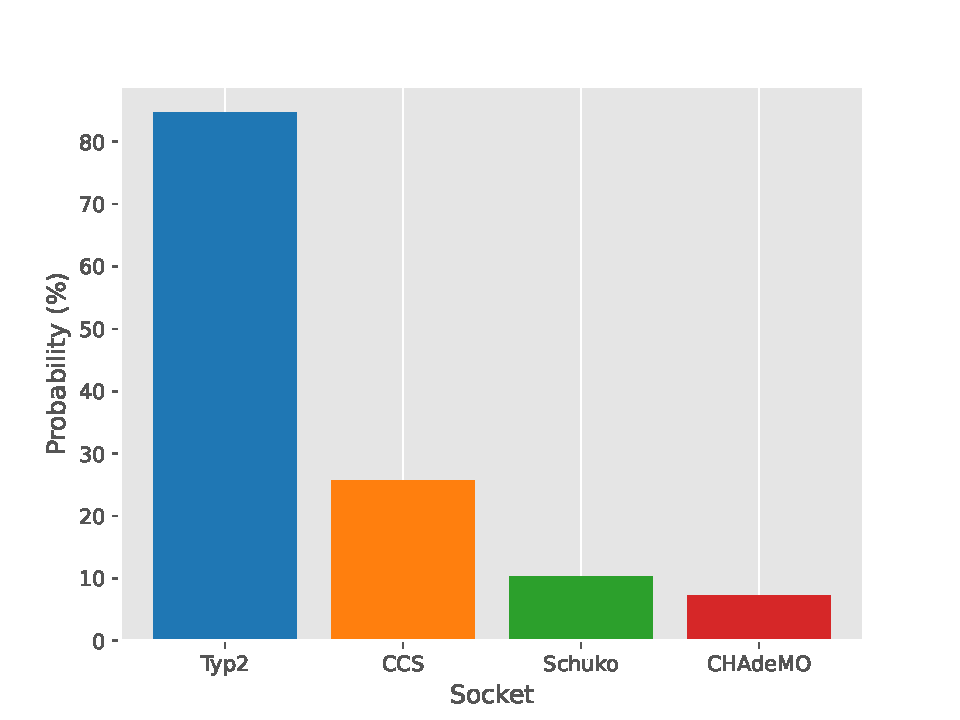
\includegraphics[width=.489\textwidth]{graphs/socket_probability.pdf}
    \caption{Probability to find socket X at a random charging location}
    \label{fig:socketsprob}
\end{figure}



\section{Charging Station Architectures}
% TODO: explain proposed architectures
%% \cite{acharya_cybersecurity_2020} - very good architecture schematic of grid/charging station/EV connections and communication.

\subsection{Proposed architectures}
%% \cite{deb_review_2021} - DC bus architektur
\subsection{Integration of battery storage and photovoltaics}
% TODO
\subsection{Independent charging stations}
% TODO: alpitronic
\subsection{DC Bus Systems}
% TODO: Tesla v4

\section{Attack Vectors and Impact}
%% \cite{bao_threat_2018} - ISO15118 threat analysis
%% \cite{kohler_brokenwire_2023} - jamming powerline in ISO15118 communication
%% \cite{nasr_chargeprint_2023} - framework for backend service security analysis

% impact:
%% \cite{sanghvi_cybersecurity_2021} - energy simulation using OpenDSS - impact of vulnerabilities
%% \cite{acharya_cybersecurity_2020} - very good architecture schematic of grid/charging station/EV connections and communication.

% TODO: subsections

\section{Cybersecurity State}
%% \cite{sklyar_chargepoint_nodate} - pentest of chargepoint charging station: many text-book vulnerabilities / buffer overflows / linux fails (suid bit, ssh rev tunnel to mothership, ...)

\section{Conclusion}
%% \cite{mccarthy_cybersecurity_2023} - NIST guidelines for IT security measures in EVs / charging stations / ... - as a recommendation?

\printbibliography
\end{document}
